% Figure 2 v4 — ABM Stage B + C, pictographic (icons over formulas)
% No top ribbon, no ensemble, no outputs — only what happens inside the loop.

\documentclass[border=8pt]{standalone}

\usepackage[T1]{fontenc}
\usepackage{lmodern}
\usepackage{amsmath, amssymb}
\usepackage{tikz}
\usepackage{xcolor}

\usetikzlibrary{
  positioning, arrows.meta, shapes.geometric, calc, fit, backgrounds,
  decorations.pathmorphing,
}

\definecolor{stageBBg}     {HTML}{FCE4C7}
\definecolor{stageBBanner} {HTML}{C2410C}
\definecolor{stageCBg}     {HTML}{F5E6D8}
\definecolor{stageCBanner} {HTML}{92400E}
\definecolor{cFlow}        {HTML}{E07A5F}
\definecolor{cBPR}         {HTML}{F59E0B}
\definecolor{cText}        {HTML}{1F2937}
\definecolor{cMuted}       {HTML}{6B7280}
\definecolor{cAgentWalk}   {HTML}{10B981}
\definecolor{cAgentTransit}{HTML}{F59E0B}
\definecolor{cAgentCar}    {HTML}{3B82F6}
\definecolor{cTierLow}     {HTML}{93C5FD}
\definecolor{cTierMid}     {HTML}{C4B5FD}
\definecolor{cTierHigh}    {HTML}{F0ABFC}

\begin{document}

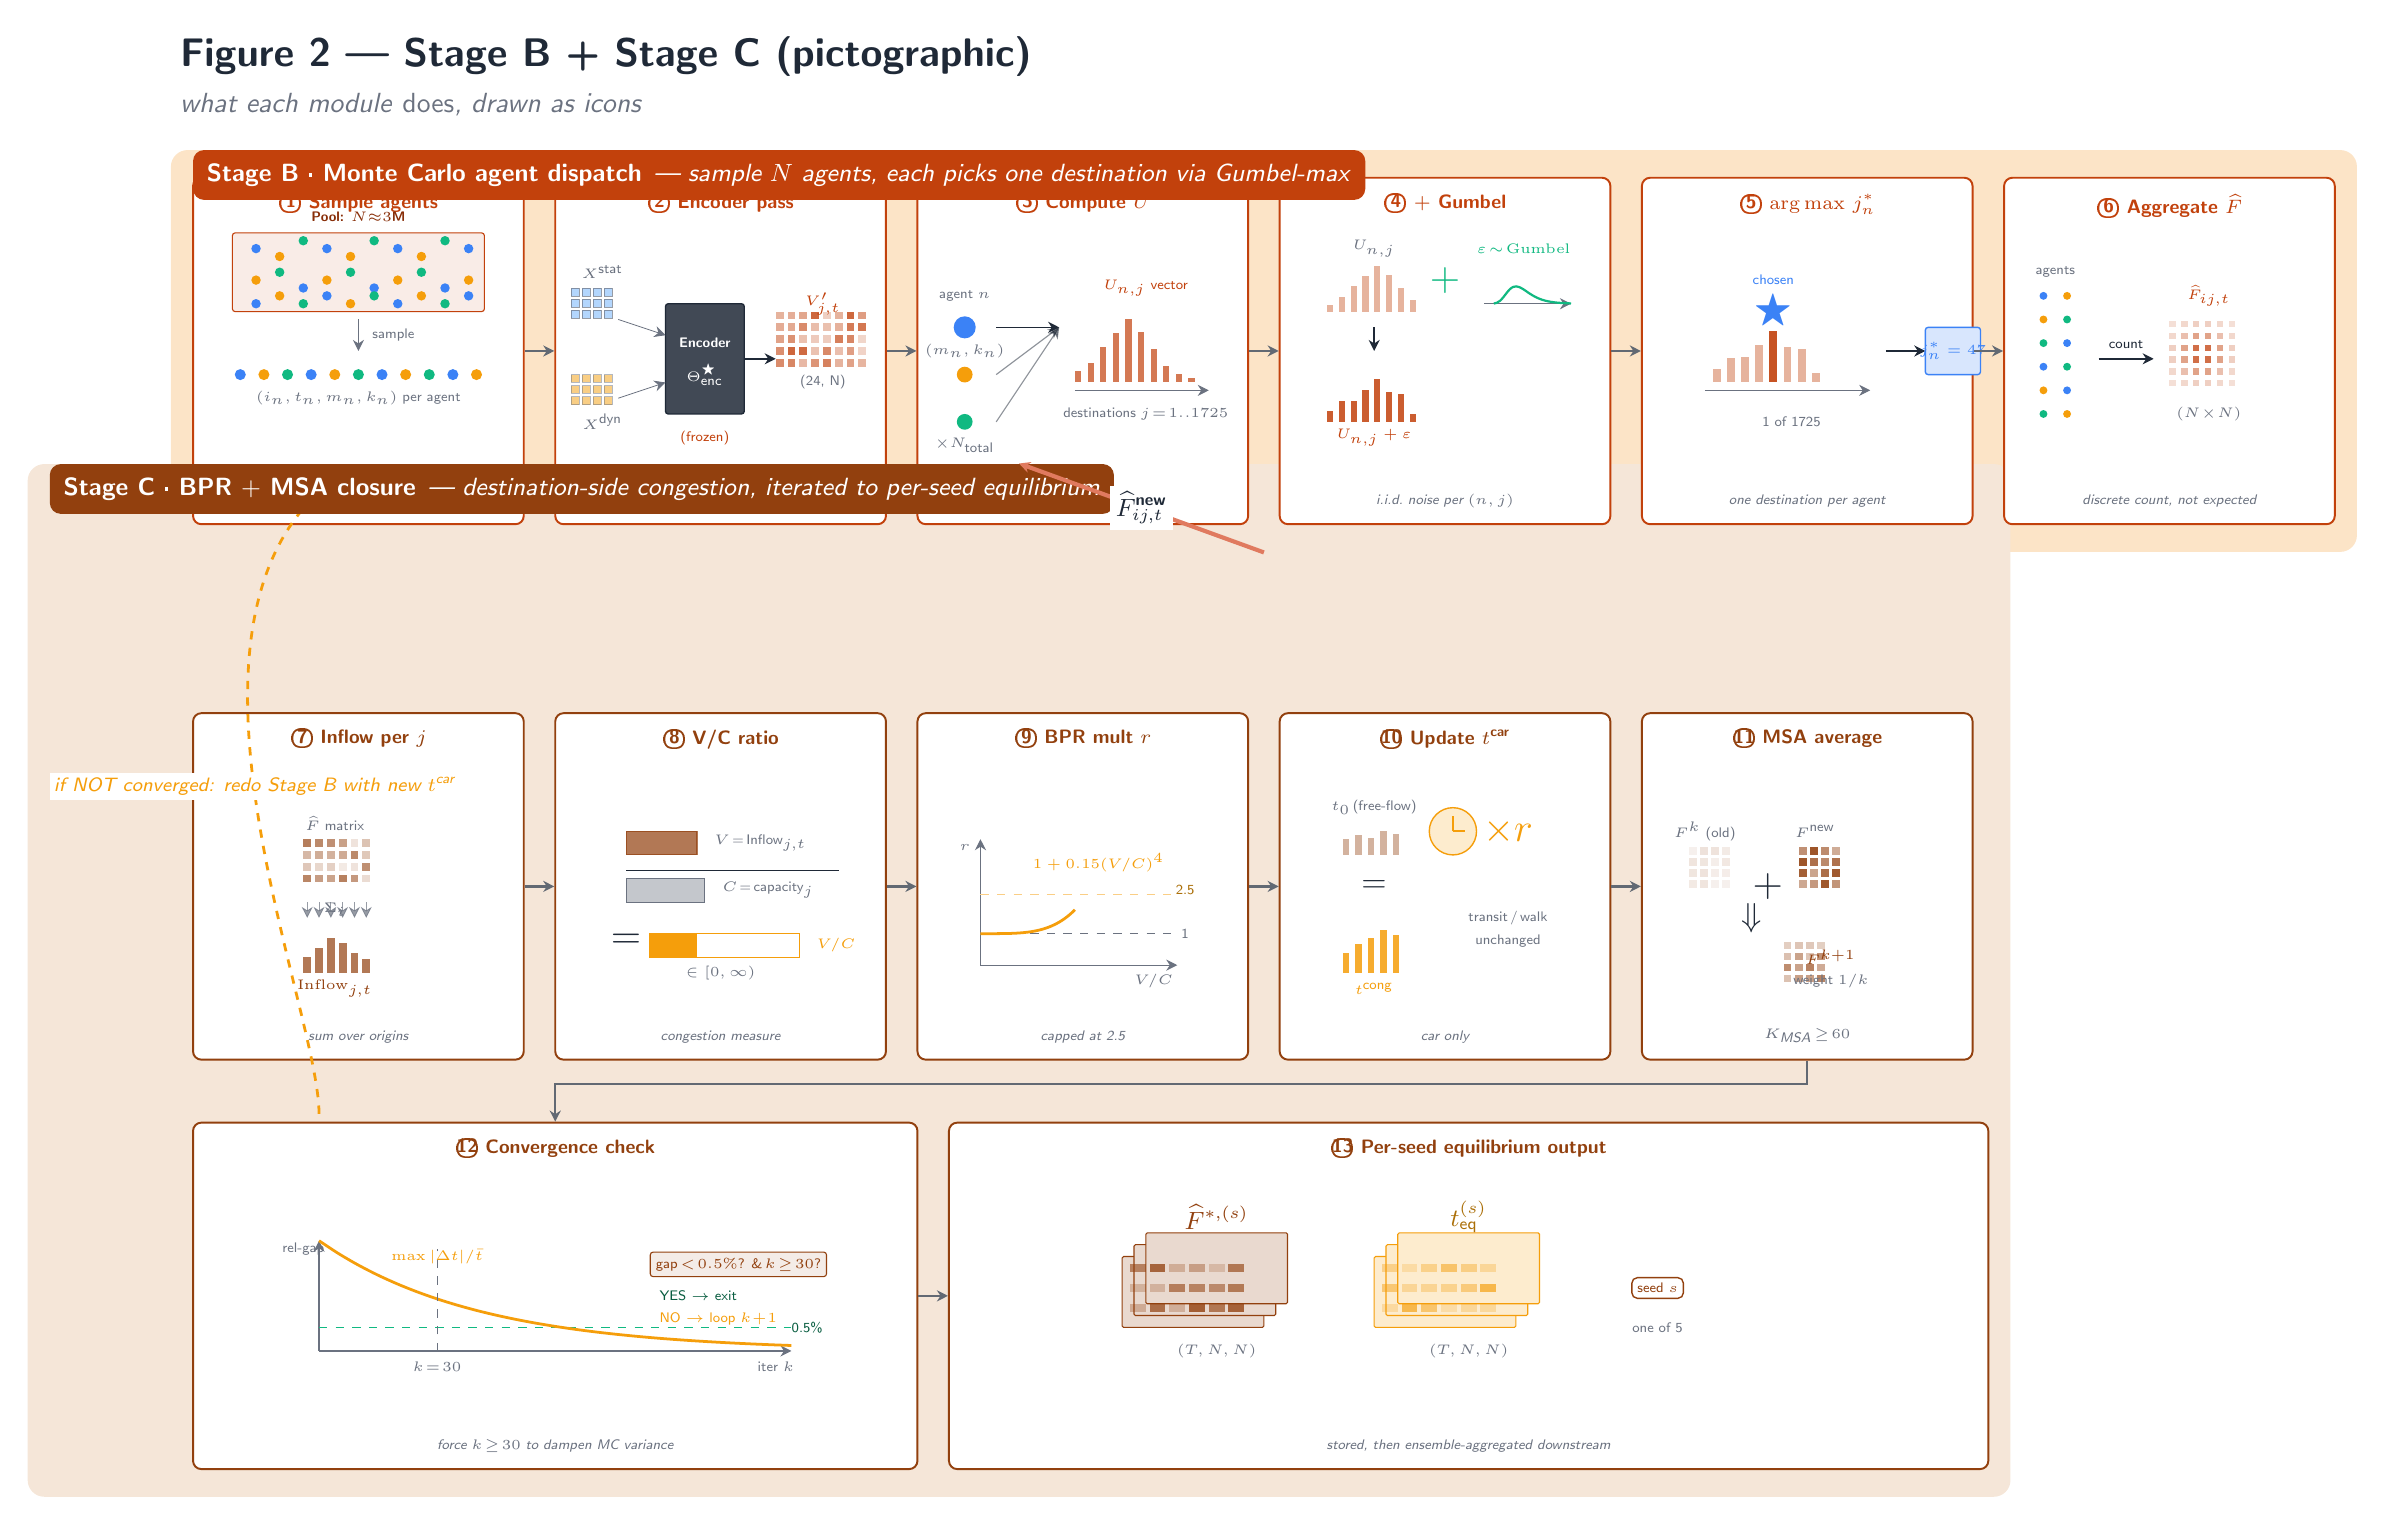
\begin{tikzpicture}[
  font=\sffamily\footnotesize,
  >={Stealth[length=4pt, width=4pt]},
  every node/.style={align=center, text=cText},
  rowframe/.style={
    draw=none, fill=#1, rounded corners=6pt,
    inner xsep=8pt, inner ysep=10pt,
  },
  rowbanner/.style={
    fill=#1, text=white, font=\sffamily\bfseries\small,
    rounded corners=4pt, inner sep=5pt,
  },
  modB/.style={
    draw=stageBBanner, fill=white, line width=0.7pt,
    rounded corners=3pt, minimum width=42mm, minimum height=44mm,
    anchor=north west,
  },
  modC/.style={
    draw=stageCBanner, fill=white, line width=0.7pt,
    rounded corners=3pt, minimum width=42mm, minimum height=44mm,
    anchor=north west,
  },
  arrInner/.style={->, line width=0.9pt, draw=cText!70},
  arrBPR/.style={->, line width=1.0pt, draw=cBPR, dashed},
  arrFwd/.style={->, line width=1.5pt, draw=cFlow},
  modtitle/.style={
    font=\sffamily\bfseries\scriptsize, text=#1, anchor=north,
  },
  modcap/.style={
    font=\sffamily\tiny\itshape, text=cMuted, anchor=south,
  },
]

% ════════════════════════════════════════════════════════════════════════
%  STAGE B · 6 MODULES (single row)
% ════════════════════════════════════════════════════════════════════════

\begin{scope}[local bounding box=stageB]

  % ────────────────────────────────────────────────────────────────────
  %  ① Sample N tuples  — pool of agents with (mode, tier) tagging
  % ────────────────────────────────────────────────────────────────────
  \node[modB] (m1) at (0, 0) {};
  \node[modtitle=stageBBanner] at ($(m1.north)+(0,-1mm)$)
       {\textcircled{\scriptsize 1}\;Sample agents};

  \begin{scope}[shift={($(m1.center)+(0, 1mm)$)}]
    % large pool rectangle at top with dots
    \draw[draw=stageBBanner, fill=stageBBanner!10, rounded corners=1pt, line width=0.4pt]
        (-16mm, 4mm) rectangle (16mm, 14mm);
    \foreach \dx/\dy/\col in
        {-13/12/cAgentCar, -10/11/cAgentTransit, -7/13/cAgentWalk,
         -4/12/cAgentCar, -1/11/cAgentTransit, 2/13/cAgentWalk,
         5/12/cAgentCar, 8/11/cAgentTransit, 11/13/cAgentWalk, 14/12/cAgentCar,
         -13/8/cAgentTransit, -10/9/cAgentWalk, -7/7/cAgentCar,
         -4/8/cAgentTransit, -1/9/cAgentWalk, 2/7/cAgentCar,
         5/8/cAgentTransit, 8/9/cAgentWalk, 11/7/cAgentCar, 14/8/cAgentTransit,
         -13/5/cAgentCar, -10/6/cAgentTransit, -7/5/cAgentWalk,
         -4/6/cAgentCar, -1/5/cAgentTransit, 2/6/cAgentWalk,
         5/5/cAgentCar, 8/6/cAgentTransit, 11/5/cAgentWalk, 14/6/cAgentCar}{
      \fill[\col] (\dx mm, \dy mm) circle (0.6mm);
    }
    \node[font=\sffamily\tiny, text=stageBBanner!70!black]
         at (0, 16mm) {\textbf{Pool: $N{\approx}3$M}};

    % "draw" arrow
    \draw[->, line width=0.5pt, draw=cMuted] (0, 3mm) -- (0, -1mm)
         node[midway, right, font=\sffamily\tiny, text=cMuted] {\;sample};

    % bottom row: tagged agents
    \foreach \i/\dx/\col/\sh in {
       0/-15/cAgentCar/c, 1/-12/cAgentTransit/t, 2/-9/cAgentWalk/w,
       3/-6/cAgentCar/c, 4/-3/cAgentTransit/t, 5/0/cAgentWalk/w,
       6/3/cAgentCar/c, 7/6/cAgentTransit/t, 8/9/cAgentWalk/w,
       9/12/cAgentCar/c, 10/15/cAgentTransit/t}{
      \fill[\col] (\dx mm, -4mm) circle (0.7mm);
    }
    \node[font=\sffamily\tiny, text=cMuted] at (0, -7mm)
         {\textbf{$(i_n,t_n,m_n,k_n)$} per agent};
  \end{scope}

  \node[modcap] at ($(m1.south)+(0, 1mm)$)
       {drawn from $\pi_m(i)\!\cdot\!\pi_k(i)$};

  % ────────────────────────────────────────────────────────────────────
  %  ② Encoder pass — features → black box → V heatmap
  % ────────────────────────────────────────────────────────────────────
  \node[modB] (m2) at (46mm, 0) {};
  \node[modtitle=stageBBanner] at ($(m2.north)+(0,-1mm)$)
       {\textcircled{\scriptsize 2}\;Encoder pass};

  \begin{scope}[shift={($(m2.center)+(0, -1mm)$)}]
    % static features (top-left)
    \foreach \r in {0,1,2}{
      \foreach \c in {0,1,2,3}{
        \draw[fill=cTierLow, opacity=0.7, draw=cMuted, line width=0.2pt]
              (-19mm + \c*1.4mm, 8mm - \r*1.4mm) rectangle
              (-18mm + \c*1.4mm, 9mm - \r*1.4mm);
      }
    }
    \node[font=\sffamily\tiny, text=cMuted] at (-15mm, 11mm) {$X^\text{stat}$};

    % dynamic features (bottom-left)
    \foreach \r in {0,1,2}{
      \foreach \c in {0,1,2,3}{
        \draw[fill=cAgentTransit, opacity=0.5, draw=cMuted, line width=0.2pt]
              (-19mm + \c*1.4mm, -3mm - \r*1.4mm) rectangle
              (-18mm + \c*1.4mm, -2mm - \r*1.4mm);
      }
    }
    \node[font=\sffamily\tiny, text=cMuted] at (-15mm, -8mm) {$X^\text{dyn}$};

    % black box
    \draw[draw=cText, fill=cText!85, rounded corners=1pt, line width=0.5pt]
          (-7mm, -7mm) rectangle (3mm, 7mm);
    \node[font=\sffamily\tiny\bfseries, text=white] at (-2mm, 2mm) {Encoder};
    \node[font=\sffamily\tiny, text=white] at (-2mm, -2mm) {$\Theta_\text{enc}^{\bigstar}$};
    \node[font=\sffamily\tiny, text=stageBBanner] at (-2mm, -10mm) {(frozen)};

    % arrow into box
    \draw[->, line width=0.3pt, draw=cMuted] (-13mm, 5mm) -- (-7mm, 3mm);
    \draw[->, line width=0.3pt, draw=cMuted] (-13mm, -5mm) -- (-7mm, -3mm);

    % output V heatmap (right)
    \foreach \r in {0,1,2,3,4}{
      \foreach \c in {0,1,2,3,4,5,6,7}{
        \pgfmathsetmacro{\op}{0.2 + 0.6*rnd}
        \fill[stageBBanner, opacity=\op]
              (7mm + \c*1.5mm, 5mm - \r*1.5mm) rectangle
              (8mm + \c*1.5mm, 6mm - \r*1.5mm);
      }
    }
    \draw[->, line width=0.5pt, draw=cText] (3mm, 0mm) -- (7mm, 0mm);
    \node[font=\sffamily\tiny, text=stageBBanner] at (13mm, 7mm) {$V'_{j,t}$};
    \node[font=\sffamily\tiny, text=cMuted] at (13mm, -3mm) {(24, N)};
  \end{scope}

  \node[modcap] at ($(m2.south)+(0, 1mm)$)
       {1$\times$ vectorised forward};

  % ────────────────────────────────────────────────────────────────────
  %  ③ Compute U for each agent — agent → utility bar chart
  % ────────────────────────────────────────────────────────────────────
  \node[modB] (m3) at (92mm, 0) {};
  \node[modtitle=stageBBanner] at ($(m3.north)+(0,-1mm)$)
       {\textcircled{\scriptsize 3}\;Compute $U$};

  \begin{scope}[shift={($(m3.center)+(0, -1mm)$)}]
    % single agent (large dot) at left
    \fill[cAgentCar] (-15mm, 4mm) circle (1.4mm);
    \node[font=\sffamily\tiny, text=cMuted] at (-15mm, 8mm) {agent $n$};
    \node[font=\sffamily\tiny, text=cMuted] at (-15mm, 1mm) {$(m_n,k_n)$};

    % arrow with multiple lines (representing many agents)
    \draw[->, line width=0.6pt, draw=cText] (-11mm, 4mm) -- (-3mm, 4mm);
    \fill[cAgentTransit] (-15mm, -2mm) circle (1.0mm);
    \draw[->, line width=0.4pt, draw=cText, opacity=0.5] (-11mm, -2mm) -- (-3mm, 4mm);
    \fill[cAgentWalk] (-15mm, -8mm) circle (1.0mm);
    \draw[->, line width=0.4pt, draw=cText, opacity=0.5] (-11mm, -8mm) -- (-3mm, 4mm);
    \node[font=\sffamily\tiny, text=cMuted] at (-15mm, -11mm) {$\times N_\text{total}$};

    % U bars over destinations
    \foreach \k/\h in {0/1.0, 1/1.8, 2/3.2, 3/4.5, 4/5.8, 5/4.6, 6/3.0, 7/1.5, 8/0.8, 9/0.4}{
      \fill[stageBBanner, opacity=0.7]
            (-1mm + \k*1.6mm, -3mm) rectangle
            (-0.2mm + \k*1.6mm, -3mm + \h*1.4mm);
    }
    \draw[->, line width=0.3pt, draw=cMuted] (-1mm, -4mm) -- (16mm, -4mm);
    \node[font=\sffamily\tiny, text=cMuted] at (8mm, -7mm) {destinations $j\!=\!1..1725$};
    \node[font=\sffamily\tiny, text=stageBBanner] at (8mm, 9mm) {$U_{n,j}$ vector};
  \end{scope}

  \node[modcap] at ($(m3.south)+(0, 1mm)$)
       {GPU-batched over agents};

  % ────────────────────────────────────────────────────────────────────
  %  ④ Add Gumbel ε  — bars + curve = noisy bars
  % ────────────────────────────────────────────────────────────────────
  \node[modB] (m4) at (138mm, 0) {};
  \node[modtitle=stageBBanner] at ($(m4.north)+(0,-1mm)$)
       {\textcircled{\scriptsize 4}\;$+$ Gumbel};

  \begin{scope}[shift={($(m4.center)+(0, -1mm)$)}]
    % U bars (background)
    \foreach \k/\h in {0/0.8, 1/1.8, 2/3.2, 3/4.5, 4/5.8, 5/4.6, 6/3.0, 7/1.5}{
      \fill[stageBBanner, opacity=0.4]
            (-15mm + \k*1.5mm, 6mm) rectangle
            (-14.2mm + \k*1.5mm, 6mm + \h*1.0mm);
    }
    \node[font=\sffamily\tiny, text=cMuted] at (-9mm, 14mm) {$U_{n,j}$};

    % plus
    \node[font=\sffamily\Large, text=cAgentWalk] at (0mm, 10mm) {$+$};

    % Gumbel curve
    \draw[->, line width=0.3pt, draw=cMuted] (5mm, 7mm) -- (16mm, 7mm);
    \draw[cAgentWalk, line width=0.8pt, smooth, samples=25, domain=-2:5]
          plot ({\x*1.4mm + 9mm}, {6mm * exp(-\x - exp(-\x)) + 7mm});
    \node[font=\sffamily\tiny, text=cAgentWalk] at (10mm, 14mm) {$\varepsilon\!\sim\!\mathrm{Gumbel}$};

    % equal arrow
    \draw[->, line width=0.5pt, draw=cText] (-9mm, 4mm) -- (-9mm, 1mm);

    % U + ε bars (foreground, perturbed heights)
    \foreach \k/\h in {0/1.4, 1/2.6, 2/2.7, 3/4.0, 4/5.5, 5/3.8, 6/3.5, 7/1.0}{
      \fill[stageBBanner, opacity=0.85]
            (-15mm + \k*1.5mm, -8mm) rectangle
            (-14.2mm + \k*1.5mm, -8mm + \h*1.0mm);
    }
    \node[font=\sffamily\tiny, text=stageBBanner] at (-9mm, -10mm) {$U_{n,j} + \varepsilon$};
  \end{scope}

  \node[modcap] at ($(m4.south)+(0, 1mm)$)
       {i.i.d.\ noise per $(n,j)$};

  % ────────────────────────────────────────────────────────────────────
  %  ⑤ argmax j*  — bars with star on max
  % ────────────────────────────────────────────────────────────────────
  \node[modB] (m5) at (184mm, 0) {};
  \node[modtitle=stageBBanner] at ($(m5.north)+(0,-1mm)$)
       {\textcircled{\scriptsize 5}\;$\arg\max\,j_n^*$};

  \begin{scope}[shift={($(m5.center)+(0, -2mm)$)}]
    % bars with star on max
    \foreach \k/\h/\chosen in
        {0/1.4/0, 1/2.6/0, 2/2.7/0, 3/4.0/0, 4/5.5/1,
         5/3.8/0, 6/3.5/0, 7/1.0/0}{
      \pgfmathsetmacro{\op}{0.4 + 0.5*\chosen}
      \fill[stageBBanner, opacity=\op]
            (-12mm + \k*1.8mm, -2mm) rectangle
            (-11mm + \k*1.8mm, -2mm + \h*1.2mm);
    }
    % star
    \node[font=\sffamily\Large, text=cAgentCar] at (-12mm + 4*1.8mm + 0.5mm, 7mm)
         {$\bigstar$};
    \node[font=\sffamily\tiny, text=cAgentCar] at (-12mm + 4*1.8mm + 0.5mm, 11mm)
         {chosen};

    \draw[->, line width=0.3pt, draw=cMuted] (-13mm, -3mm) -- (8mm, -3mm);

    % output: single dest j*
    \draw[->, line width=0.7pt, draw=cText] (10mm, 2mm) -- (15mm, 2mm);
    \draw[draw=cAgentCar, fill=cAgentCar!20, rounded corners=1pt, line width=0.5pt]
          (15mm, -1mm) rectangle (22mm, 5mm);
    \node[font=\sffamily\tiny, text=cAgentCar] at (18.5mm, 2mm) {$j_n^* = 47$};

    \node[font=\sffamily\tiny, text=cMuted] at (-2mm, -7mm) {1 of 1725};
  \end{scope}

  \node[modcap] at ($(m5.south)+(0, 1mm)$)
       {one destination per agent};

  % ────────────────────────────────────────────────────────────────────
  %  ⑥ Aggregate F̂  — many agents → flow heatmap
  % ────────────────────────────────────────────────────────────────────
  \node[modB] (m6) at (230mm, 0) {};
  \node[modtitle=stageBBanner] at ($(m6.north)+(0,-1mm)$)
       {\textcircled{\scriptsize 6}\;Aggregate $\widehat{F}$};

  \begin{scope}[shift={($(m6.center)+(0, -1mm)$)}]
    % many tiny agents on left, all feeding into 2D grid
    \foreach \dx/\dy/\col in {
        -16/8/cAgentCar, -16/5/cAgentTransit, -16/2/cAgentWalk,
        -16/-1/cAgentCar, -16/-4/cAgentTransit, -16/-7/cAgentWalk,
        -13/8/cAgentTransit, -13/5/cAgentWalk, -13/2/cAgentCar,
        -13/-1/cAgentWalk, -13/-4/cAgentCar, -13/-7/cAgentTransit}{
      \fill[\col] (\dx mm, \dy mm) circle (0.5mm);
    }
    \node[font=\sffamily\tiny, text=cMuted] at (-14.5mm, 11mm) {agents};

    % arrow with "count"
    \draw[->, line width=0.5pt, draw=cText] (-9mm, 0mm) -- (-2mm, 0mm)
         node[midway, above, font=\sffamily\tiny, text=cText] {count};

    % output: F̂ heatmap (i × j)
    \foreach \r in {0,1,2,3,4,5}{
      \foreach \c in {0,1,2,3,4,5}{
        \pgfmathsetmacro{\op}{0.15 + 0.7*exp(-((\r-2.5)*(\r-2.5) + (\c-2.5)*(\c-2.5))*0.3)}
        \fill[stageBBanner, opacity=\op]
              (0mm + \c*1.5mm, 4mm - \r*1.5mm) rectangle
              (0.8mm + \c*1.5mm, 4.8mm - \r*1.5mm);
      }
    }
    \node[font=\sffamily\tiny, text=stageBBanner] at (5mm, 8mm) {$\widehat{F}_{ij,t}$};
    \node[font=\sffamily\tiny, text=cMuted] at (5mm, -7mm) {$(N\!\times\!N)$};
  \end{scope}

  \node[modcap] at ($(m6.south)+(0, 1mm)$)
       {discrete count, not expected};

  % inner arrows
  \draw[arrInner] (m1.east) -- (m2.west);
  \draw[arrInner] (m2.east) -- (m3.west);
  \draw[arrInner] (m3.east) -- (m4.west);
  \draw[arrInner] (m4.east) -- (m5.west);
  \draw[arrInner] (m5.east) -- (m6.west);

\end{scope}

\begin{pgfonlayer}{background}
  \node[rowframe=stageBBg, fit=(stageB)] (frameStageB) {};
\end{pgfonlayer}
\node[rowbanner=stageBBanner, anchor=north west]
  at ($(frameStageB.north west)+(8pt, 0pt)$)
  {\textsc{Stage B · Monte Carlo agent dispatch}\;\,\textmd{\itshape — sample $N$ agents, each picks one destination via Gumbel-max}};

% ════════════════════════════════════════════════════════════════════════
%  STAGE C · 7 MODULES (5 in row 1, 2 in row 2)
% ════════════════════════════════════════════════════════════════════════

\begin{scope}[local bounding box=stageC, shift={(0, -68mm)}]

  % ────────────────────────────────────────────────────────────────────
  %  ⑦ Inflow per j  — F̂ matrix → column sum → bars
  % ────────────────────────────────────────────────────────────────────
  \node[modC] (n7) at (0, 0) {};
  \node[modtitle=stageCBanner] at ($(n7.north)+(0,-1mm)$)
       {\textcircled{\scriptsize 7}\;Inflow per $j$};

  \begin{scope}[shift={($(n7.center)+(0, -1mm)$)}]
    % F̂ matrix at top
    \foreach \r in {0,1,2,3}{
      \foreach \c in {0,1,2,3,4,5}{
        \pgfmathsetmacro{\op}{0.1 + 0.6*rnd}
        \fill[stageCBanner, opacity=\op]
              (-7mm + \c*1.5mm, 6mm - \r*1.5mm) rectangle
              (-6mm + \c*1.5mm, 7mm - \r*1.5mm);
      }
    }
    \node[font=\sffamily\tiny, text=cMuted] at (-3mm, 9mm) {$\widehat{F}$ matrix};

    % column-wise sum arrow
    \foreach \c in {0,1,2,3,4,5}{
      \draw[->, line width=0.3pt, draw=cMuted, opacity=0.7]
        (-6.5mm + \c*1.5mm, -1mm) -- (-6.5mm + \c*1.5mm, -3mm);
    }
    \node[font=\sffamily\tiny, text=cMuted] at (-3mm, -2mm) {$\Sigma_i$};

    % bars output (inflow per j)
    \foreach \c/\h in {0/2.0, 1/3.2, 2/4.5, 3/3.8, 4/2.6, 5/1.8}{
      \fill[stageCBanner, opacity=0.7]
            (-7mm + \c*1.5mm, -10mm) rectangle
            (-6mm + \c*1.5mm, -10mm + \h*1.0mm);
    }
    \node[font=\sffamily\tiny, text=stageCBanner] at (-3mm, -12mm) {$\mathrm{Inflow}_{j,t}$};
  \end{scope}

  \node[modcap] at ($(n7.south)+(0, 1mm)$)
       {sum over origins};

  % ────────────────────────────────────────────────────────────────────
  %  ⑧ V/C ratio  — inflow / capacity = ratio gauge
  % ────────────────────────────────────────────────────────────────────
  \node[modC] (n8) at (46mm, 0) {};
  \node[modtitle=stageCBanner] at ($(n8.north)+(0,-1mm)$)
       {\textcircled{\scriptsize 8}\;V/C ratio};

  \begin{scope}[shift={($(n8.center)+(0, -1mm)$)}]
    % numerator: inflow bar
    \draw[fill=stageCBanner, opacity=0.7, draw=stageCBanner, line width=0.4pt]
        (-12mm, 5mm) rectangle (-3mm, 8mm);
    \node[font=\sffamily\tiny, text=cMuted, anchor=west] at (-2mm, 6.5mm)
         {$V$\,=\,Inflow$_{j,t}$};

    % divide line
    \draw[draw=cText, line width=0.6pt] (-12mm, 3mm) -- (15mm, 3mm);

    % denominator: capacity bar
    \draw[fill=cMuted!40, draw=cMuted, line width=0.4pt]
        (-12mm, -1mm) rectangle (-2mm, 2mm);
    \node[font=\sffamily\tiny, text=cMuted, anchor=west] at (-1mm, 0.5mm)
         {$C$\,=\,capacity$_j$};

    % equal sign + thermometer
    \node[font=\sffamily\Large, text=cText] at (-12mm, -6mm) {$=$};
    \draw[draw=cBPR, line width=0.5pt] (-9mm, -8mm) rectangle (10mm, -5mm);
    \fill[cBPR] (-9mm, -8mm) rectangle (-3mm, -5mm);
    \node[font=\sffamily\tiny, text=cBPR, anchor=west] at (11mm, -6.5mm)
         {$V/C$};
    \node[font=\sffamily\tiny, text=cMuted] at (0mm, -10mm)
         {$\in [0, \infty)$};
  \end{scope}

  \node[modcap] at ($(n8.south)+(0, 1mm)$)
       {congestion measure};

  % ────────────────────────────────────────────────────────────────────
  %  ⑨ BPR multiplier — convex curve plot
  % ────────────────────────────────────────────────────────────────────
  \node[modC] (n9) at (92mm, 0) {};
  \node[modtitle=stageCBanner] at ($(n9.north)+(0,-1mm)$)
       {\textcircled{\scriptsize 9}\;BPR mult $r$};

  \begin{scope}[shift={($(n9.center)+(-3mm, -3mm)$)}]
    % axes
    \draw[->, line width=0.4pt, draw=cMuted] (-10mm, -7mm) -- (15mm, -7mm);
    \draw[->, line width=0.4pt, draw=cMuted] (-10mm, -7mm) -- (-10mm, 9mm);
    \node[font=\sffamily\tiny, text=cMuted] at (12mm, -9mm) {$V/C$};
    \node[font=\sffamily\tiny, text=cMuted] at (-12mm, 8mm) {$r$};

    % horizontal line at r=1 (free flow)
    \draw[draw=cMuted, dashed, line width=0.3pt] (-10mm, -7mm + 4mm) -- (15mm, -7mm + 4mm);
    \node[font=\sffamily\tiny, text=cMuted] at (16mm, -3mm) {1};

    % cap line at r=2.5
    \draw[draw=cBPR!50, dashed, line width=0.3pt] (-10mm, -7mm + 9mm) -- (15mm, -7mm + 9mm);
    \node[font=\sffamily\tiny, text=cBPR!70!black] at (16mm, 2.5mm) {2.5};

    % BPR curve
    \draw[cBPR, line width=1.0pt, smooth, samples=25, domain=0:1.5]
          plot ({-10mm + \x*8mm}, {-7mm + (1 + 0.15*\x*\x*\x*\x)*4mm});
    \node[font=\sffamily\tiny, text=cBPR] at (5mm, 6mm) {$1+0.15(V/C)^4$};
  \end{scope}

  \node[modcap] at ($(n9.south)+(0, 1mm)$)
       {capped at 2.5};

  % ────────────────────────────────────────────────────────────────────
  %  ⑩ Update t_car  — bars × multiplier, with clock icon
  % ────────────────────────────────────────────────────────────────────
  \node[modC] (n10) at (138mm, 0) {};
  \node[modtitle=stageCBanner] at ($(n10.north)+(0,-1mm)$)
       {\textcircled{\scriptsize 10}\;Update $t^\text{car}$};

  \begin{scope}[shift={($(n10.center)+(0, -1mm)$)}]
    % free-flow times bar chart
    \foreach \k/\h in {0/2.0, 1/2.5, 2/2.2, 3/3.0, 4/2.7}{
      \fill[stageCBanner, opacity=0.4]
            (-13mm + \k*1.6mm, 5mm) rectangle
            (-12.2mm + \k*1.6mm, 5mm + \h*1.0mm);
    }
    \node[font=\sffamily\tiny, text=cMuted] at (-9mm, 11mm) {$t_0$\,(free-flow)};

    % clock icon
    \draw[draw=cBPR, fill=cBPR!20, line width=0.5pt] (1mm, 8mm) circle (3mm);
    \draw[cBPR, line width=0.6pt] (1mm, 8mm) -- (1mm, 10mm);
    \draw[cBPR, line width=0.6pt] (1mm, 8mm) -- (2.5mm, 8mm);

    % multiplier annotation
    \node[font=\sffamily\Large, text=cBPR] at (8mm, 8mm) {$\times r$};

    % equal sign
    \node[font=\sffamily\large, text=cText] at (-9mm, 1mm) {$=$};

    % congested times (longer)
    \foreach \k/\h in {0/2.6, 1/3.7, 2/4.4, 3/5.5, 4/4.8}{
      \fill[cBPR, opacity=0.85]
            (-13mm + \k*1.6mm, -10mm) rectangle
            (-12.2mm + \k*1.6mm, -10mm + \h*1.0mm);
    }
    \node[font=\sffamily\tiny, text=cBPR] at (-9mm, -12mm) {$t^\text{cong}$};
    \node[font=\sffamily\tiny, text=cMuted] at (8mm, -3mm) {transit\,/\,walk};
    \node[font=\sffamily\tiny, text=cMuted] at (8mm, -6mm) {unchanged};
  \end{scope}

  \node[modcap] at ($(n10.south)+(0, 1mm)$)
       {car only};

  % ────────────────────────────────────────────────────────────────────
  %  ⑪ MSA averaging — old + new = blended
  % ────────────────────────────────────────────────────────────────────
  \node[modC] (n11) at (184mm, 0) {};
  \node[modtitle=stageCBanner] at ($(n11.north)+(0,-1mm)$)
       {\textcircled{\scriptsize 11}\;MSA average};

  \begin{scope}[shift={($(n11.center)+(0, -1mm)$)}]
    % F^old (faded)
    \foreach \r in {0,1,2,3}{
      \foreach \c in {0,1,2,3}{
        \pgfmathsetmacro{\op}{0.1 + 0.4*rnd}
        \fill[stageCBanner, opacity={0.2 * \op + 0.05}]
              (-15mm + \c*1.4mm, 5mm - \r*1.4mm) rectangle
              (-14mm + \c*1.4mm, 6mm - \r*1.4mm);
      }
    }
    \node[font=\sffamily\tiny, text=cMuted] at (-13mm, 8mm) {$F^k$ (old)};

    % plus
    \node[font=\sffamily\Large, text=cText] at (-5mm, 1mm) {$+$};

    % F^new (bright)
    \foreach \r in {0,1,2,3}{
      \foreach \c in {0,1,2,3}{
        \pgfmathsetmacro{\op}{0.4 + 0.5*rnd}
        \fill[stageCBanner, opacity=\op]
              (-1mm + \c*1.4mm, 5mm - \r*1.4mm) rectangle
              (0mm + \c*1.4mm, 6mm - \r*1.4mm);
      }
    }
    \node[font=\sffamily\tiny, text=cMuted] at (1mm, 8mm) {$F^\text{new}$};

    % equal arrow
    \node[font=\sffamily\large, text=cText] at (-7mm, -3mm) {$\Downarrow$};

    % blended
    \foreach \r in {0,1,2,3}{
      \foreach \c in {0,1,2,3}{
        \pgfmathsetmacro{\op}{0.25 + 0.4*rnd}
        \fill[stageCBanner, opacity=\op]
              (-3mm + \c*1.4mm, -7mm - \r*1.4mm) rectangle
              (-2mm + \c*1.4mm, -6mm - \r*1.4mm);
      }
    }
    \node[font=\sffamily\tiny, text=stageCBanner] at (3mm, -8mm) {$F^{k+1}$};
    \node[font=\sffamily\tiny, text=cMuted] at (3mm, -11mm) {weight $1/k$};
  \end{scope}

  \node[modcap] at ($(n11.south)+(0, 1mm)$)
       {$K_\text{MSA}\!\geq\!60$};

  % ────────────────────────────────────────────────────────────────────
  %  ⑫ Convergence check — line graph approaching threshold
  % ────────────────────────────────────────────────────────────────────
  \node[modC, minimum width=92mm] (n12) at (0, -52mm) {};
  \node[modtitle=stageCBanner] at ($(n12.north)+(0,-1mm)$)
       {\textcircled{\scriptsize 12}\;Convergence check};

  \begin{scope}[shift={($(n12.center)+(0, 0)$)}]
    % axes
    \draw[->, line width=0.4pt, draw=cMuted] (-30mm, -7mm) -- (30mm, -7mm);
    \draw[->, line width=0.4pt, draw=cMuted] (-30mm, -7mm) -- (-30mm, 7mm);
    \node[font=\sffamily\tiny, text=cMuted] at (28mm, -9mm) {iter $k$};
    \node[font=\sffamily\tiny, text=cMuted] at (-32mm, 6mm) {rel-gap};

    % threshold line at 0.5%
    \draw[draw=cAgentWalk, dashed, line width=0.5pt] (-30mm, -4mm) -- (30mm, -4mm);
    \node[font=\sffamily\tiny, text=cAgentWalk!50!black] at (32mm, -4mm) {0.5\%};

    % rel-gap curve (decreasing)
    \draw[cBPR, line width=1.0pt, smooth, samples=25, domain=0:1]
          plot ({-30mm + \x*60mm}, {-7mm + 14mm * exp(-3*\x)});
    \node[font=\sffamily\tiny, text=cBPR] at (-15mm, 5mm) {$\max|\Delta t|/\bar{t}$};

    % "k=30 enforce" mark
    \draw[draw=cMuted, dashed, line width=0.3pt] (-15mm, -7mm) -- (-15mm, 6mm);
    \node[font=\sffamily\tiny, text=cMuted] at (-15mm, -9mm) {$k\!=\!30$};

    % decision diamond
    \node[font=\sffamily\tiny, text=stageCBanner, anchor=west,
           draw=stageCBanner, fill=stageCBanner!10, rounded corners=1pt,
           line width=0.4pt, inner sep=2pt] at (12mm, 4mm)
         {gap\,$<\!0.5\%$? \&\,$k\!\geq\!30$?};
    \node[font=\sffamily\tiny, text=cAgentWalk!50!black, anchor=west] at (12mm, 0mm)
         {YES $\to$ exit};
    \node[font=\sffamily\tiny, text=cBPR, anchor=west] at (12mm, -3mm)
         {NO $\to$ loop $k\!+\!1$};
  \end{scope}

  \node[modcap] at ($(n12.south)+(0, 1mm)$)
       {force $k\!\geq\!30$ to dampen MC variance};

  % ────────────────────────────────────────────────────────────────────
  %  ⑬ Per-seed output  — labelled tensor pair
  % ────────────────────────────────────────────────────────────────────
  \node[modC, minimum width=132mm] (n13) at (96mm, -52mm) {};
  \node[modtitle=stageCBanner] at ($(n13.north)+(0,-1mm)$)
       {\textcircled{\scriptsize 13}\;Per-seed equilibrium output};

  \begin{scope}[shift={($(n13.center)+(0, -1mm)$)}]
    % F* tensor (left)
    \foreach \layer in {0,1,2}{
      \draw[draw=stageCBanner, fill=stageCBanner!20, line width=0.4pt, rounded corners=0.5pt]
            (-44mm + \layer*1.5mm, -3mm + \layer*1.5mm)
            rectangle
            (-26mm + \layer*1.5mm, 6mm + \layer*1.5mm);
    }
    \foreach \r in {0,1,2}{
      \foreach \c in {0,1,2,3,4,5}{
        \pgfmathsetmacro{\op}{0.2 + 0.6*rnd}
        \fill[stageCBanner, opacity=\op]
              (-43mm + \c*2.5mm, 4mm - \r*2.5mm) rectangle
              (-41mm + \c*2.5mm, 5mm - \r*2.5mm);
      }
    }
    \node[font=\sffamily\small, text=stageCBanner] at (-32mm, 11mm)
         {$\widehat{F}^{*,(s)}$};
    \node[font=\sffamily\tiny, text=cMuted] at (-32mm, -6mm) {$(T,N,N)$};

    % t_eq tensor (right)
    \foreach \layer in {0,1,2}{
      \draw[draw=cBPR, fill=cBPR!20, line width=0.4pt, rounded corners=0.5pt]
            (-12mm + \layer*1.5mm, -3mm + \layer*1.5mm)
            rectangle
            (6mm + \layer*1.5mm, 6mm + \layer*1.5mm);
    }
    \foreach \r in {0,1,2}{
      \foreach \c in {0,1,2,3,4,5}{
        \pgfmathsetmacro{\op}{0.2 + 0.5*rnd}
        \fill[cBPR, opacity=\op]
              (-11mm + \c*2.5mm, 4mm - \r*2.5mm) rectangle
              (-9mm + \c*2.5mm, 5mm - \r*2.5mm);
      }
    }
    \node[font=\sffamily\small, text=cBPR!70!black] at (0mm, 11mm)
         {$t_\text{eq}^{(s)}$};
    \node[font=\sffamily\tiny, text=cMuted] at (0mm, -6mm) {$(T,N,N)$};

    % seed s tag
    \node[draw=stageCBanner, fill=white, rounded corners=2pt, line width=0.5pt,
           font=\sffamily\tiny, text=stageCBanner, inner sep=2pt]
          at (24mm, 2mm) {seed $s$};
    \node[font=\sffamily\tiny, text=cMuted] at (24mm, -3mm) {one of 5};
  \end{scope}

  \node[modcap] at ($(n13.south)+(0, 1mm)$)
       {stored, then ensemble-aggregated downstream};

  % inner arrows row 1
  \draw[arrInner] (n7.east) -- (n8.west);
  \draw[arrInner] (n8.east) -- (n9.west);
  \draw[arrInner] (n9.east) -- (n10.west);
  \draw[arrInner] (n10.east) -- (n11.west);

  % row 1 → row 2 transition
  \draw[arrInner] (n11.south) -- ++(0, -3mm) -| (n12.north);

  % row 2 internal
  \draw[arrInner] (n12.east) -- (n13.west);

  % BPR feedback loop (orange dashed) from ⑫ back to ② (Stage B encoder)
  \draw[arrBPR] ($(n12.north)+(-30mm, 1mm)$) .. controls
                 ($(n12.north)+(-30mm, 14mm)$) and
                 ($(n12.north)+(-50mm, 60mm)$) ..
                 node[fill=white, font=\sffamily\scriptsize\itshape, text=cBPR,
                      inner sep=1.5pt, pos=0.55]
                     {if NOT converged: redo Stage B with new $t^\text{car}$}
                 ($(n12.north)+(-30mm, 80mm)$);

\end{scope}

\begin{pgfonlayer}{background}
  \node[rowframe=stageCBg, fit=(stageC)] (frameStageC) {};
\end{pgfonlayer}
\node[rowbanner=stageCBanner, anchor=north west]
  at ($(frameStageC.north west)+(8pt, 0pt)$)
  {\textsc{Stage C · BPR $+$ MSA closure}\;\,\textmd{\itshape — destination-side congestion, iterated to per-seed equilibrium}};

% main forward arrow from B to C
\draw[arrFwd] ($(frameStageB.south)+(0, 0)$) --
              node[fill=white, font=\sffamily\bfseries\small,
                   text=cText, inner sep=2pt]
                  {$\widehat{F}_{ij,t}^\text{new}$}
              ($(frameStageC.north)+(0, 0)$);

% Title
\node[font=\sffamily\bfseries\Large, anchor=south west, text=cText]
  at ($(frameStageB.north west)+(0, 8mm)$)
  {Figure 2 — Stage B + Stage C (pictographic)};
\node[font=\sffamily\itshape\normalsize, anchor=south west, text=cMuted]
  at ($(frameStageB.north west)+(0, 3mm)$)
  {what each module \emph{does}, drawn as icons};

\end{tikzpicture}

\end{document}
